\chapter{Turbulence}\label{turbulence}
The equations for a general compressible, viscous, selfgravitating fluid 
with density $\rho(r_i,t)$, momentum density $\rho v_i(r_i,t)$ and total
energy density $\rho e(r_i,t)$ are\footnote{see eg. \citet{Landau1991}.}
\begin{align}
\pd{t}\rho + \pd{r_j}(v_j \rho) &= 0, \label{eq:mass}\\
\pd{t}(\rho v_i) + \pd{r_j}(v_j \rho v_i) &= -\pd{r_i}p + \pd{r_j}\sigma'_{ij}
+\rho g_i, 
\label{eq:mom} \\
\pd{t}(\rho e) + \pd{r_j}(v_j \rho e) &= -\pd{r_j}(v_j p) + \pd{r_j}(v_i
\sigma'_{ij}) + v_i \rho g_i,
\label{eq:etot}
\end{align}
with Newtonian gravity (Poisson Equation)
\begin{align}
\pd{r_j}g_j=4\pi G \rho
\end{align}
and an equation of state to compute the pressure $p(r_i,t)$ dependent on
the material of the fluid. For a Newtonian fluid the stress tensor
$\sigma_{ij}$ is of the form\footnote{For a derivation see Appendix
\ref{stress}.}
\begin{align}
\sigma'_{ij} =  
2\eta\lrb{\frac{1}{2}\lra{\ppd{r_j}{v_i}+\ppd{r_i}{v_j}}
-\frac{1}{3}\delta_{ij}\ppd{r_k}{v_k}}
+\zeta \delta_{ij}\ppd{r_k}{v_k},
\end{align}
where the so called dynamic viscosity $\eta$ and the second viscosity $\zeta$
are defined to be constants\footnote{The literature on incompressible flows
often defines the so called kinematic viscosity $\nu=\frac{\eta}{\rho}$. It
should be noted, that this quantity is a constant only for fluids of constant
density and cannot be used in a meaningful way when discussing compressible
flows.} in a Newtonian fluid.

This system of differential equations is complex and highly nonlinear if the
nonlinear advection term $\pd{r_j}(v_j \rho v_i)$ dominates in the momentum
equation \eqref{eq:mom} and in general can be solved only numerically.
The influence of the advection term can be estimated by writing down the 
momentum equation in dimensionless form, which yields\footnote{See Appendix
\ref{dimanal}.}
\begin{align}
\underbrace{\frac{l_0}{v_0 t_0}}_{Sr}\pd{t^*}(\rho^* v_i^*) 
+ \pd{r_j^*}(v_j^* \rho^* v_i^*) &= 
-\underbrace{\frac{p_0}{\rho_0 v_0^2}}_{Ma^{-2}_{iso}}\pd{r_i^*}p^* 
+\underbrace{\frac{\sigma_0}{\rho_0 v_0^2}}_{Re^{-1}}\pd{r_j^*}\sigma_{ij}^*
+\underbrace{\frac{\rho_0 g_0 l_0}{\rho_0 v_0^2}}_{Fr^{-1}} \rho^* g_i^*.
\end{align}
The arising dimensionless numbers\footnote{The Strouhal number
 $Sr$ can be set to one by assuming $v_0=\frac{l_0}{t_0}$.}
($Re$ = Reynolds number, $Ma_{iso}$ =
isothermal Mach number, and $Fr$ = Froude number)
show the ratio of the mean pressure energy density $p_0$, the
mean potential energy density $\rho_0 g_0 l_0$, and the mean energy dissipation
density $\sigma_0$ to the mean kinetic energy density $\rho_0 v_0^2$. 
If all these numbers are much greater than one (which means the mean
kinetic energy is big compared to the other energies), the advection term
dominates and the fluid flow is called turbulent. 

\section{Phenomenology of Turbulence}
As there is no accepted theory of compressible, selfgravitating turbulence we
have to restrict the following discussion to incompressible turbulence. For an
incompressible fluid, it can be shown that the Reynolds number
\begin{align}
Re=\frac{\rho_0 v_0^2}{\sigma_0}=\frac{\rho_0 l_0 v_0}{\eta_0} 
\end{align}
is the only number which characterizes the dynamics of the fluid flow
\citep{Feynman1964}. 

\begin{figure}[tp]
\centering
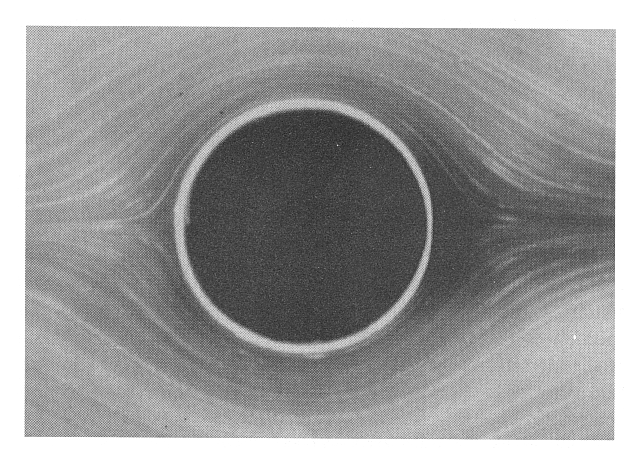
\includegraphics[width=0.7\linewidth]{chapter2/Reynolds0.eps}
\caption{Laminar flow past a cylinder at $Re=0.16$ \citep{Frisch1995}.}
\label{fig:rey0}
\end{figure}

If the Reynolds numbers is small, which is the case for high viscosity and/or
low flow speed, we call the fluid laminar. In this laminar state the streamlines
of the fluid exhibit all the symmetries of the equations and boundary
conditions. This can be seen in figure \ref{fig:rey0}, where the streamlines of
a fluid around a cylinder show up-down and left-right symmetry.\footnote{
Actually the streamlines also show z-invariance (along the axes of the cylinder)
and time-invariance, but they do not show cylindrical symmetry as the direction
of the fluid flow breaks this symmetry.} 

\begin{figure}[tp]
	\centering
	\subfigure[$Re=240$]
	{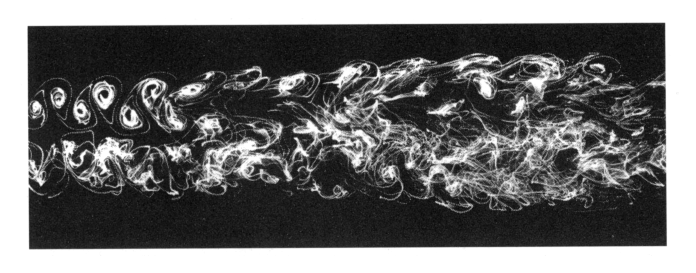
\includegraphics[width=0.7\linewidth]{chapter2/Reynolds240.eps}
	\label{fig:rey240}}
	\subfigure[$Re=1800$]
	{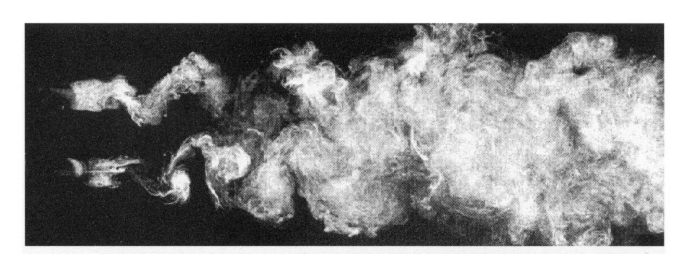
\includegraphics[width=0.7\linewidth]{chapter2/Reynolds1800.eps}
	\label{fig:rey1800}}
	\caption{Wake behind two identical cylinders \citep{Frisch1995}.}
\end{figure}


With increasing Reynolds number,
the left-right symmetry first (figure \;\ref{fig:rey240}) and then the up-down
symmetry are broken (figure \;\ref{fig:rey1800}). If $Re > 1000$, the flow
becomes completely chaotic and all symmetries are broken. Nevertheless, looking
at the flow at smaller scales $l$ far from the boundaries, all the symmetries of
the equations seem to be restored in a statistical sense. This state of flow is
called fully developed turbulence.

However at the smallest scales of the flow $l_k$,
the flow will ``behave'' laminar again. This means that the Reynolds
number becomes smaller on smaller scales and implies that the Reynolds number is
scale dependent
\begin{align}
Re(l)=\frac{\rho v(l) l}{\eta}. 
\end{align}
How the Reynolds number depends on the scales of the flow is explained by the
Kolmogorov theory of incompressible turbulence.

\section{The Kolmogorov theory}\label{kolmo}
Kolmogorov first described his theory of turbulence in 1941. 
Here we discuss the modern formulation of the Kolmogorov theory as
explained in \citet{Frisch1995} and \citet{Pope2000}.

According to Frisch, Kolmogorovs theory is based on three
assumptions which are valid in the limit of infinite Reynolds numbers, at small
scales $l$ $(l_k \ll l \ll l_0)$ and away from boundaries:
\begin{enumerate}
\item All the possible symmetries of
the Navier-Stokes equation, usually broken by the mechanisms producing the
turbulent flow, are restored in a statistical sense.
\item The turbulent flow is self-similar.
\item The turbulent flow has a finite nonvanishing mean rate of dissipation
$\fil{\epsilon}$ per unit mass.
\end{enumerate}
The mean rate of dissipation is defined as the mean rate of change of kinetic
energy
\begin{align}
\fil{\epsilon}=\fil{\td{t}e_{kin}} \sim \frac{v_0^2}{l_0/v_0} =
\frac{v_0^3}{l_0} = const. \label{eq:diss}
\end{align}
Using this Kolmogorov derived, that for homogeneous and isotropic
incompressible turbulence the third order structure function\footnote{For a
definition of structure functions see
appendix \ref{structfunc}.} $S_3(v(l))$ is equal
to the mean rate of dissipation times minus four-fifths the length scale $l$ of
the structure function
\begin{align}
S_3(v(l)) = -\frac{4}{5} \fil{\epsilon} l.
\end{align}
This is the famous four-fifths law of Kolmogorov. From
it and the self similarity assumption, Kolmogorov deduces that the structure
functions of order $p$ scale like
\begin{align}
S_p(v(l)) \sim \fil{\epsilon}^{p/3} l^{p/3}.
\end{align}
Because the second order structure function can be expressed as
Fourier transform of the longitudinal velocity
spectrum\footnote{Also see appendix \ref{structfunc}.} $\abs{V_{\parallel}(k)}^2
\sim e_{kin}(k)$ and the wave numbers $k$ are related to length scales $l$ via
$k \sim l^{-1}$ it follows for the specific kinetic energy in Fourier space
\begin{align}
e_{kin}(k) \sim \fil{\epsilon}^{2/3} k^{-2/3}. 
\end{align}
The energy spectrum $E(k)$ is the kinetic energy in
the wave number interval between $k$ and $k+dk$, which is then
\begin{align}
E(k) \sim \td{k} e_{kin}(k) = C_k \fil{\epsilon}^{2/3} k^{-5/3}.
\end{align}
This is the celebrated result of Kolmogorovs theory of incompressible
turbulence. The constant $C_k$ is therefore called the Kolmogorov constant and
is 
experimentally and numerically found to be $C_k \approx 1.6$
\citep{Yokokawa2002}. 

It should be noted that the rate of dissipation $\fil{\epsilon}$ is not the rate
of conversion of kinetic energy into internal energy, rather it describes the
amount
of energy which is transfered from the bigger to the smaller scales, without
the influence of viscosity. The kinetic energy is converted to internal energy
only on scales smaller than the Kolmogorov scale $l_k$, where the
Reynolds number becomes unity. From this and the relation $S_1(v(l)) \sim v(
l) \sim \fil{\epsilon}^{1/3} l^{1/3}$ we can derive an expression for the
Kolmogorov scale
\begin{align}
Re(l_k) = 1 = \frac{\rho v_{l_k} l_k}{\eta} = 
\frac{\fil{\epsilon}^{1/3} l_k^{4/3}}{\nu} \Rightarrow
l_k = \lra{\frac{\nu^3}{\fil{\epsilon}}}^{1/4}. \label{eq:lk}
\end{align}

Using the definition of the dissipation \eqref{eq:diss} in \eqref{eq:lk}, we
obtain for the ratio between the largest integral length $l_0$ and the
Kolmogorov length $l_k$
\begin{align}
\frac{l_0}{l_k}=\lra{\frac{\nu^3}{l_0^3 v_0^3}}^{-1/4} = Re^{3/4}. 
\end{align}
We can use this to estimate the number of degrees of freedom of a
three-dimensional fluid flow at a point of time
\begin{align}
N_f=\lra{\frac{l_0}{l_k}}^3 = Re^{9/4}.
\end{align}
One consequence of this is that the storage requirement of a fully resolved
numerical simulation grows as $Re^{9/4}$. \footnote{
Using this to estimate the Reynolds number from the biggest direct numerical
simulation today by \citet{Yokokawa2002} on the Earth simulator with a
resolution of $4096^3$ grid cells yields $Re \approx 65536$.} Since the time
step must usually be taken proportional to the spatial mesh, the total number
of operations to integrate the equations for a fixed number of dynamical times
is
\begin{align}
N = \lra{\frac{l_0}{l_k}}^4 = Re^3.
\end{align}
As the typical Reynolds numbers in astrophysical context are of the order of
$10^8$ \citep{Kritsuk2007} up to $10^{14}$ \citep{Schmidt2006} we would
need a computer with at least $10^{18}$ Bytes (1 Exabyte) of memory and
$10^{16}$ FLOPS\footnote{Floating point operations per second.} (10 PetaFLOPS)
running for a year to resolve fully an astrophysical simulation. And even
if we could efficiently make use of the fact, that turbulence is not volume
filling at a
point of time, it remains intractable to resolve completely the turbulent
fluid dynamics encountered in astrophysics \citep{Schmidt2006}.

Therefore we can only treat explicitly a limited number of degrees of freedom,
which correspond to the largest scales of the system. The influence of the
turbulent dynamics from smaller scales onto larger scales has to be treated in a
statistical way. How the dynamics on small scales and the dynamics on large
scales are interconnected, can be seen by explicitly filtering the equations of
fluid dynamics.

  